\section{绪论}

\subsection{黑体辐射}

黑体辐射曲线为图:

\begin{figure}[H]
  \centering
  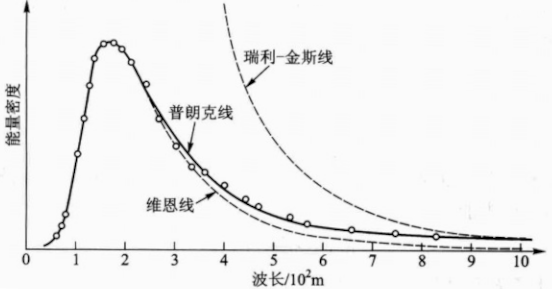
\includegraphics[width=0.65\linewidth]{figures/黑体辐射曲线}
  \caption{黑体辐射曲线}
  \label{fig:黑体辐射曲线}
\end{figure}

普朗克黑体辐射公式:

\begin{equation*}
  \begin{aligned}
    \rho_{\nu} \md \nu = \dfrac{8 \pi h \nu^3}{c^3} \cdot \dfrac{1}{\exp \left[ (h \nu) / (k_B T)  \right] - 1} \md \nu  
  \end{aligned}
\end{equation*}

其中$\rho_{\nu} \md \nu$是黑体内频率$\nu$到$\nu + \md \nu$时间辐射能量密度。

\subsection{索末菲量子化条件}

索末菲量子化条件为:

\begin{equation*}
  \begin{aligned}
    \oint p \md q = \left( n + \dfrac{1}{2}  \right) h
  \end{aligned}
\end{equation*}

$p$是广义动量,$q$是广义坐标。

%%% Local Variables:
%%% mode: latex
%%% TeX-master: "Qumntum_Mechanics"
%%% End:

